\documentclass[a4paper, 10pt, twocolumn]{article}
% Sowohl LaTeX als auch pdfLaTeX können benutzt werden, um das Manuskript zu erstellen.

% Bitte öffnen sie diese Datei mit latin1 oder ansinew Zeichenkodierung!!!
\usepackage[ansinew]{inputenc}          % Schriftkodierung dieser Datei
\usepackage[german]{babel}          % für deutsche Dokumente

\usepackage{graphicx}               % optional für Grafiken
\usepackage{tabularx}               % optional für Tabellen
\usepackage{multirow}               % optional für Tabellen
\usepackage{url}                % optional für Internet Links

\usepackage[small,bf]{caption2}     % bitte für Bildunterschriften verwenden

\usepackage{parskip}

\usepackage{titlesec}
\usepackage{amsmath}                % optional für Formeln

\titleformat{\section}{\normalfont\large\bfseries}{\thesection}{}{}
\titleformat{\subsection}{\normalfont\large\bfseries}{\thesection}{}{}
\titleformat{\paragraph}{\normalfont\bfseries}{\theparagraph}{}{}
\titlespacing{\section}{0pt}{6pt}{-1pt}
\titlespacing{\subsection}{0pt}{3pt}{-1pt}
\titlespacing{\paragraph}{0pt}{3pt}{-1pt}

\newcolumntype{Y}{>{\centering\arraybackslash}X}    %für Tabellen mit tabularx

% Definition der Seitenränder
\addtolength{\textwidth}{2.1cm}
\addtolength{\topmargin}{-2.4cm}
\addtolength{\oddsidemargin}{-1.1 cm}
\addtolength{\textheight}{4.5cm}
\setlength{\columnsep}{0.7cm}

\pagestyle{empty}                   % weder Kopf- noch Fußzeile auf 1. Seite

\begin{document}

\date{}                                         % kein Datum auf 1. Seite

\title{\vspace{-8mm}\textbf{\large
\LaTeX-Vorlage für Beiträge zur DAGA-Tagung }}


% Hier die Namen und Daten der beteiligten Autoren eintragen
\author{
Heiner Hesse$^1$, Bert Klang$^2$\\
$^1$ \emph{\small Institut für Akustik, 12345 Stadt,
Deutschland, Email: anna.schall@stadt.de
}\\
$^2$ \emph{\small Akustik-Firma GmbH, 12345 Stadt, Deutschland,
Email: akustik@firma.com } } \maketitle


\thispagestyle{empty}           % weder Kopf- noch Fußzeile auf Folgeseiten
% Beginn des eigentlichen Manuskripts
\section*{Einleitung}
\label{sec:Einleitung} Dies ist die Formatvorlage, um einen Beitrag
für den Tagungsband der DAGA zu verfassen. Um ein einheitliches
Erscheinungsbild der Beiträge im Tagungsband bzw. auf der Tagungs-CD-ROM
sicherzustellen, möchten wir Sie bitten, die hier vorgegebenen Formatvorgaben
einzuhalten und die entsprechenden Templates zu verwenden. Diese Datei enthält
die Richtlinien zur Erstellung von Beiträgen mit \LaTeX. Eine Formatvorlage
für die Beitragserstellung mit MS-Word steht auf
\url{https://www.daga2021.eu/} ebenfalls zum Download
bereit.

Die Formatvorlage stellt die nötigen Absatz- und Schrift\-einstellungen zur Verfügung, damit das Layout Ihres Beitrags so einfach wie möglich gestaltet werden kann. Bitte benutzen Sie keine Formatierungen, die nicht innerhalb dieses Templates angeboten werden. Nur so kann sicher gestellt werden, dass sämtliche Beiträge des Tagungsbandes ein einheitliches Erscheinungsbild aufweisen.

Die Manuskripte können bis zu vier Seiten enthalten.
 
Sollten Sie Ihren Beitrag auf Englisch präsentiert haben und einen englischsprachigen Titel genutzt haben, so verfassen Sie bitte auch Ihr Manuskript auf Englisch.


\section*{Wichtig}
\label{sec:Wichtig} Beim Einreichen Ihres Abstracts über die

DAGA-Homepage werden Informationen bezüglich Ihres Beitrags in
einer Datenbank abgelegt. Dies sind insbesondere:
\begin{itemize}
    \item[-] der Titel Ihres Beitrags,
    \item[-] die Liste der Autoren.
\end{itemize}
Diese Informationen werden vom System genutzt, um automatisch zum Beispiel das Tagungsprogramm, einen Autorenindex, die Tagungs-CD-ROM zu erstellen.

Es ist \textbf{besonders wichtig}, dass die Datenbank, die die Beiträge verwaltet, keine Fehler enthält und mit den Informationen in Ihrem endgültigen Manuskript übereinstimmt. Dies betrifft im Besonderen den Titel Ihres Beitrags und die Daten der beteiligten Autoren (Anzahl, Reihenfolge \ldots).

\begin{figure}[hbt]
    \begin{center}
        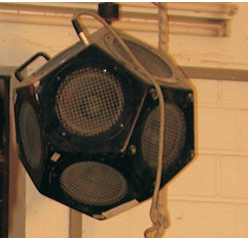
\includegraphics[width=4.2cm]{dode}
    \end{center}
    \caption{Dies ist ein Dodekaeder-Lautsprecher. Bildunterschriften sollten soviel Information enthalten, dass die zugehörige Abbildung ohne Lesen des gesamten Manuskriptes verstanden werden kann.}
    \label{fig:dode}
\end{figure}
Der Web-Server erzeugt die endgültigen Dateien, indem die eingereichten Dateien automatisch verändert werden. Dies schließt folgendes ein:
\begin{itemize}
    \item[-] Einfügen von Kopf- und Fußzeilen,
    \item[-] Einfügen der Seitenzahlen,
    \item[-] Gegebenfalls die Konvertierung in eine PDF-Datei.
\end{itemize}
Aus diesem Grund ist es \textbf{sehr wichtig}, dass Sie die folgenden Regeln bei der Erstellung Ihrer Datei berücksichtigen:
\begin{itemize}
    \item[-] \textbf{fügen Sie keinerlei Kopf- oder Fußzeilen ein,}
    \item[-] \textbf{fügen Sie keine Seitenzahlen ein,}
    \item[-] \textbf{beachten Sie die unten angegebenen Maße für Seitenränder,}
    \item[-] falls Sie die Testversion einer Software zum Erstellen Ihres PDF-Files verwendet haben, \textbf{vergewissern Sie sich, dass die Software keine
    zusätzlichen Kommentare in Ihr Dokument eingefügt hat} (Dies kann auf jeder Seite, nur auf der ersten oder letzten Seite Ihres Manuskripts der Fall
    sein).
\end{itemize}
Die eingereichten bzw. konvertierten PDF-Dateien können vor dem Erstellen des Tagungsbandes und der Tagungs-CD-ROM überprüft und verändert werden. Die Organisatoren der Tagung behalten sich vor, PDF-Dateien, die die Vorgaben nicht einhalten, abzulehnen oder entsprechend anzupassen. \textbf{Im Falle einer Ablehnung können die Autoren das Manuskript überarbeiten, so dass es den Vorgaben entspricht. Sonst wird das eingereichte Manuskript durch die zugehörige Kurzfassung ersetzt.}
\section*{Grundlegende Formatvorgaben}
\label{sec:BasicFormats}
\subsection*{Seitenlayout}
\textbf{Seitenränder:} Oben und unten jeweils 2 cm Abstand, links und rechts 1,5 cm. Der Zeilenabstand soll 0,7 cm betragen.

\textbf{Papiergröße:} A4
\subsection*{Formate}
Times New Roman ist als Standard Schriftart zu verwenden.

\textbf{Titel:} Die Vorgaben dieses Templates sind beizubehalten.

\textbf{Autoren:} Die Vorgaben dieses Templates sind beizubehalten.

\textbf{Institution:} Die Vorgaben dieses Templates sind beizubehalten.
\paragraph*{Überschriften} Benutzen Sie bitte die folgenden Befehle, um Überschriften zu definieren: section*, subsection*, und paragraph*.
\paragraph*{Textkörper} Schreiben Sie einfach drauf los.
\section*{Spezielle Formatvorgaben}
\label{sec:SpecialFormats}
\subsection*{Grafiken}
Beschriftungen von Grafiken und Abbildungen werden als Unterschrift zentriert in der Mitte der betreffenden Spalte eingefügt (wie bei Abbildungen~\ref{fig:dode} und \ref{fig:Erwin}). Benutzen Sie das Package caption2, um Bildunterschriften zu definieren.
\begin{figure}[htb]
    \begin{center}
        
\includegraphics[width=4cm]{Erwin}
    \end{center}
    \caption{Entdeckung des nächsten Wurmloches rechts des Andromedanebels.}
    \label{fig:Erwin}
\end{figure}
\subsection*{Tabellen}
Tabellen werden wie unten dargestellt formatiert. Die Beschriftung wird als Überschrift oberhalb der Tabelle angeordnet.
\begin{table}[htbp]
    \centering
    \caption{Das ist eine Tabelle}
    \vspace{2mm}
    \label{tab:DescriptiveTextForATable}
        \begin{tabularx}{8cm}{@{\arrayrulewidth1.5pt\vline}Y@{\arrayrulewidth1.5pt\vline}Y|Y|Y@{\arrayrulewidth1.5pt\vline}}
            \noalign{\hrule height1.5pt} \multirow{2}{*}{Variante} & \multicolumn{3}{c@{\arrayrulewidth1.5pt\vline}}{Parameter}\\
            \cline{2-4} & A & B & C \\
            \noalign{\hrule height1.5pt} X & AX & BX & CX\\
            \hline Y & AY & BY & CY\\
            \hline Z & AZ & BZ & CZ\\
            \noalign{\hrule height1.5pt}
        \end{tabularx}
\end{table}
\subsection*{Literaturverzeichnis}
Verwendete Literatur wird am Ende des Manuskripts angegeben. Artikel \cite{ArticleReference}, Bücher \cite{BookReference} und Internet-Adressen \cite{URLReference}\cite{PDFCreator}\cite{Ghostware} werden wie unter Literatur angegeben zitiert.
\subsection*{Formeln}
Gleichungen sind zu nummerieren und so anzuordnen, wie beispielsweise Gleichung~(\ref{eq:FirstEquation}).
\begin{flalign}
\label{eq:FirstEquation}
            \qquad\qquad F &= \pi r^2 & \mathrm{\left[m^2\right]} \quad
\end{flalign}
Stellen Sie sicher, dass alle vorkommenden Variablen bei der ersten Verwendung erläutert werden.\\
Benutzen Sie für Gleichungen statt der equation-Umgebung die flalign-Umgebung aus dem amsmath-Package.
\section*{Erzeugen einer PDF-Datei}
\label{sec:pdf}
Das Manuskript sollte als PDF-Datei eingereicht werden. Um eine ausreichend gute Druckqualität sicherzustellen, ist eine Auflösung von 600 dpi für den PDF-Export zu wählen.

Die folgenden Anforderungen sind zu erfüllen:
\begin{itemize}
    \item[-] Das Manuskript muss als A4 Seiten formatiert sein.
    \item[-] Das Manuskript darf nicht mehr als 4 Seiten enthalten.
    \item[-] Alle verwendeten Schriftarten \textbf{müssen} in das PDF-File eingebettet sein.
\end{itemize}
Alternativ können Word- und PostScript-Dateien eingereicht werden. Der Server konvertiert diese in eine PDF-Datei.
\subsection*{Häufige Probleme}
\textbf{A4 format:} Hauptsächlich unter UNIX formatieren einige Konvertierungsprogramme bei der Umwandlung von DVI nach PDF das Seitenformat als US Letter, selbst wenn dies in der \LaTeX-Datei als A4 vorgegeben ist. Deshalb muss beim Konvertieren ein vom Programm abhängiger Parameter zusätzlich gesetzt werden.
Alternativ kann auch pdf\LaTeX benutzt werden.

\textbf{Eingebettete Schriften:} Bei der Konfiguration von Acrobat Distiller ist darauf zu achten, dass \textbf{alle} Schriftarten eingebettet werden. Dies ist in der Regel \textbf{nicht} der Standard. Als kostenlose Alternative zu Adobe Acrobat gibt es die Software PDFCreator \cite{PDFCreator}. Desweiteren lassen sich Postscript-Dateien (*.ps) mit Hilfe von Ghostview/ Ghostscript \cite{Ghostware} in das PDF-Format umwandeln.
\begin{thebibliography}{5}
\bibitem{ArticleReference}
Schall, A.: How to write a manuscript. Acta Acustica united with
Acustica 90 (2004), 2203-2503
\bibitem{BookReference}
Klang, B.: Akustik im Überblick. Schall und Rauch Verlag, Stadt,
2010
\bibitem{URLReference}
DAGA Homepage, URL:\\
\url{http://www.daga-tagung.de/}
\bibitem{PDFCreator}
PDFCreator, URL:\\
\url{http://sourceforge.net/projects/pdfcreator}
\bibitem{Ghostware}
Free software Ghostview and Ghostscript, URL:\\
\url{http://www.cs.wisc.edu/~ghost/}
\end{thebibliography}
\end{document}
